\documentclass[]{article}
\usepackage[utf8]{inputenc}
\usepackage{pythonhighlight}
\usepackage{graphicx}

\begin{document}

\begin{abstract}
This is a fun project in a series called FridayNightSimulations or FridayNightExperiments that I started in October 2020 (Yes. This is the first fun project on record). The aim of this project is just to do something interesting to do as well as fun. This project is fitting an elephant with machine learning techniques. In this document, I will discuss the technical aspects of this fun project.

\end{abstract}


\section{Orgin of the problem}

Following is taken from an interview clip of Freeman Dyson (www.youtube.com/watch?v=hV41QEKiMlM). 
You can also see the video in webofstories.com.

Freeman Dyson wanted to show a result which he thought it was interesting. He went to Chicago and showed the graphs where Numerical data and Fermi's data. 

Fermi's reply: "I am not very impressed with what you have been doing".

When you are doing theoretical calculations, there are two ways to it. 

Either you should have a clear physical model in your mind or you should have a rigorous mathematical basis. 

Freeman Dyson asked "What about the numerical agreement"?

Fermi asked "How many parameters did you use for the fitting?(there were four)
Fermi answered "You know! John von Neumann always used to say "With four parameter, I can fit an elephant. With five, I can make him wiggle his trunk". 

So, I don't find the numerical accuracy impressive either.

This is the orgin of Fitting an elephant with four parameters.

There is a paper written on this topic and published in American Journal of Physics.: “Drawing an elephant with four complex parameters” by Jurgen Mayer, Khaled Khairy, and Jonathon Howard,  Am. J. Phys. 78, 648 (2010), DOI:10.1119/1.3254017.

In this fun project, I would like to fit an elephant with four parameters using Machine Learning techniques, probably using logistic regression.

\newpage

\section{Other Approaches}

\begin{python}

"""
Author: Piotr A. Zolnierczuk (zolnierczukp at ornl dot gov)
(Twitter page: https://twitter.com/zolnie)

Based on a paper by:
Drawing an elephant with four complex parameters
Jurgen Mayer, Khaled Khairy, and Jonathon Howard,
Am. J. Phys. 78, 648 (2010), DOI:10.1119/1.3254017
"""
import numpy as np
import pylab

# elephant parameters
p1, p2, p3, p4 = (50 - 30j, 18 +  8j, 12 - 10j, -14 - 60j )
p5 = 40 + 20j # eyepiece

def fourier(t, C):
    f = np.zeros(t.shape)
    A, B = C.real, C.imag
    for k in range(len(C)):
        f = f + A[k]*np.cos(k*t) + B[k]*np.sin(k*t)
    return f

def elephant(t, p1, p2, p3, p4, p5):
    npar = 6
    Cx = np.zeros((npar,), dtype='complex')
    Cy = np.zeros((npar,), dtype='complex')

    Cx[1] = p1.real*1j
    Cx[2] = p2.real*1j
    Cx[3] = p3.real
    Cx[5] = p4.real

    Cy[1] = p4.imag + p1.imag*1j
    Cy[2] = p2.imag*1j
    Cy[3] = p3.imag*1j

    x = np.append(fourier(t,Cx), [-p5.imag])
    y = np.append(fourier(t,Cy), [p5.imag])

    return x,y

x, y = elephant(np.linspace(0,2*np.pi,1000), p1, p2, p3, p4, p5)
pylab.plot(y,-x,'.')
pylab.show()

\end{python}

If you run this code in python, you will get following elephant-like shape \Cref{fig:elephant}.


\begin{figure}
\label{fig:elephant}
\centering
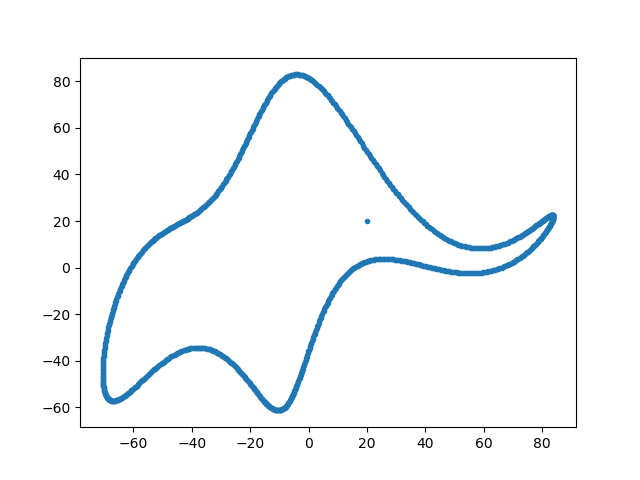
\includegraphics[width=0.8\textwidth,natwidth=610,natheight=642]{elephant.png}

\caption{This is the shape of the elephant that is plotted using the code given above.}
\end{figure}





Now, we are going to generate a lots of data from this code and we are going use logistic regression (a machine learning technique) to learn the paramerters from this and find out how  close the fitting parameters are.

\section{Packages Needed}

Python Latex Highlighting ( A package for highlighting Python code)
https://github.com/olivierverdier/python-latex-highlighting 

How to fin an elephant (JohnDCook.com)
https://www.johndcook.com/blog/2011/06/21/how-to-fit-an-elephant/

A paper has already been written on this topic and published in American Journal of Physics.
“Drawing an elephant with four complex parameters” by Jurgen Mayer, Khaled Khairy, and Jonathon Howard,  Am. J. Phys. 78, 648 (2010), DOI:10.1119/1.3254017.

I will list all the packages one by one here.

I am going to write a complete code from scratch to do this.


\section{Machine Learning Preliminaries}

What is a machine learning?
Machine learning is a method in which you teach computer to learn like us without programming explicitly. For the definition, you can find somewhere else.

Steps:

1. Generate a lots of data using this script to use as training set
2. Write ML algorithm (logistic regression)
3. Find the number of fitting parameters required with and and without lostic regression (logistic regression may reduce the number of fitting parameters required)


\end{document}
